\section{Models} \label{sec:models}
\begin{figure*}[ht]

\centering
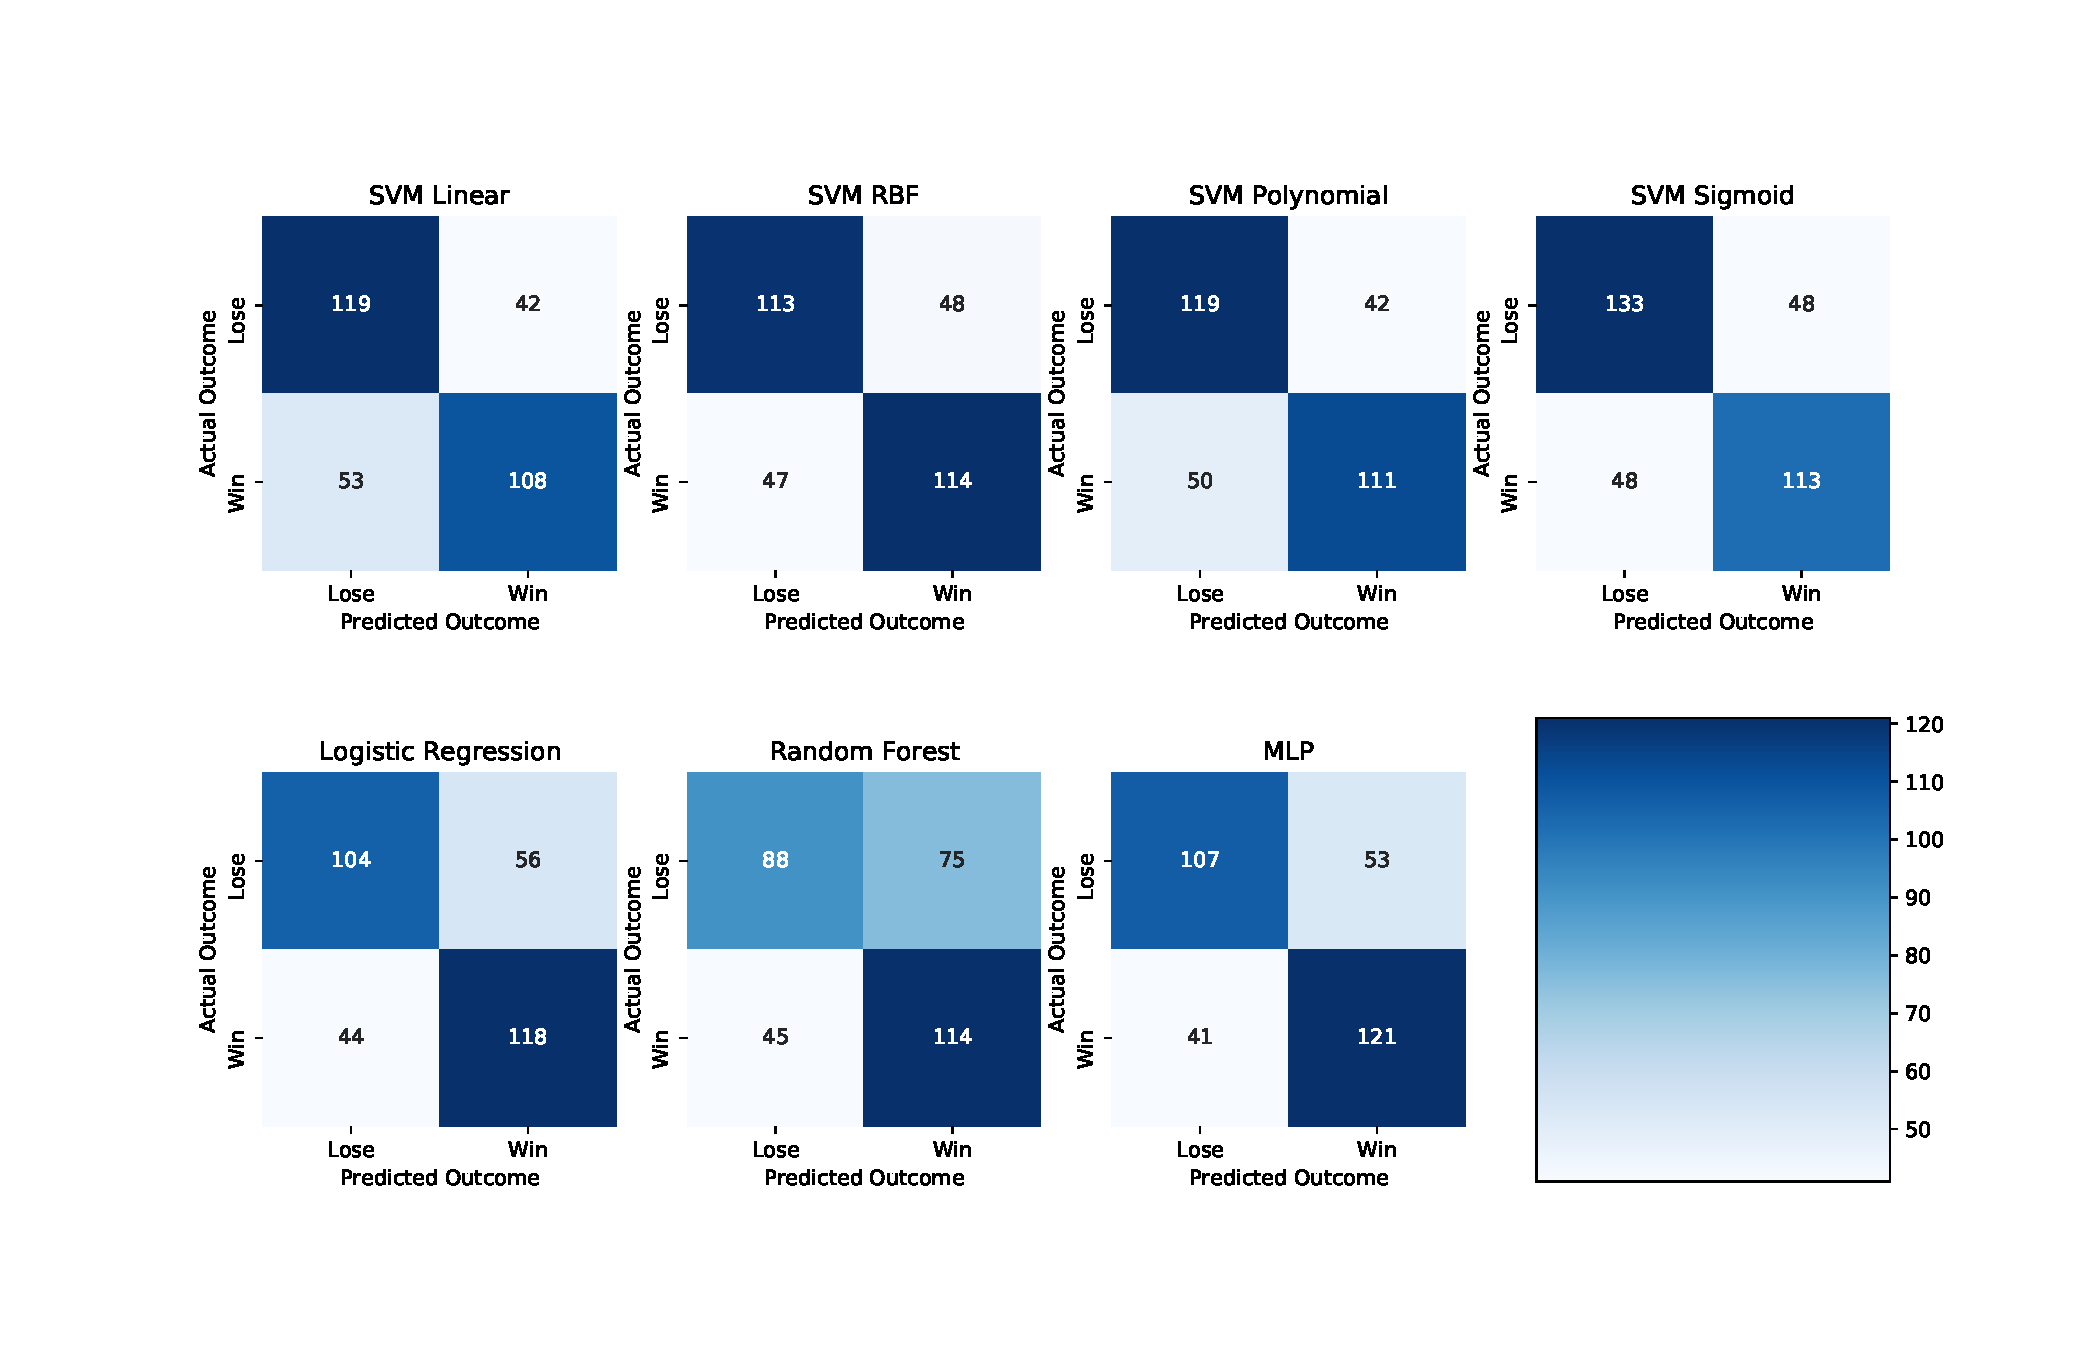
\includegraphics[width=\textwidth]{plots/confusionmatrices.pdf}
\vspace{-2em}

\caption{Confusion matrices comparing the predicted and actual outcomes of test cases for each trained model \denes{Please reduce outside margins and consider removing the legend}}

\label{fig:confusionmatricesr2}
\centering
\end{figure*}


\denes{This is where we can still cut out quit a lot if we want to}

This paper uses Scikit-Learn's implementation to apply different models to the dataset \cite{pedregosa2011scikit}.

\subsection{Logistic Regression}
The logistic function $\sigma(t)$ is defined as follows:
\begin{equation}
    \sigma(x) = \frac{1}{1+e^{-x}}
\end{equation}

The logistic function maps any input value $x$ where $x = \{x\in \mathbb{R} \}$ to a value between 0 and 1, allowing the output to be interpreted as a probability. If this probability is considered to be over 0.5, it can be classified as true, where the player is predicted to win the match, otherwise the result is classified as false. The model gives the best reproduction of match outcomes for the training set by minimising the \textit{logistic loss} function:

\begin{equation}
    (p) = -\frac{1}{n} \sum_{i=1}^n p_i \log(y_i) + (1-p_i)\log(1-y_i)
\end{equation}

$$
\begin{gathered}
    n = \text{number of matches} \\
    p_i = \text{predicted probability of a player winning match $i$} \\
    y_i = \text{outcome of match $i$},
\end{gathered}
$$

where a loss function measures the disparity between observations and their estimated fits \cite{hazan2014logistic}.

\subsection{Random Forest}
A random forest is a classifier consisting of a collection of simpler tree-structured classifiers $\{h(\textbf{x},\theta_k),\ k=1,...\}$, where the $\{\theta_k\}$ are independent identically distributed random vectors and each tree casts a unit vote for the most popular class at input $\textbf{x}$. For the $k$th tree, a random vector $\theta_k$ is generated and a tree is grown using $\theta_k$ and the training set, to produce a classifier $h(\textbf{x}, \theta_k)$ \cite{breiman2001random}. After a large number of trees are produced, the output of a random forest model is the class that receives the most votes. Decision trees tend to be simple to interpret and ``quick'' to train, making it a popular ML technique.

\subsection{Support Vector Machines (SVM)}
SVMs have been used in predicting tennis match outcome \cite{cornman2017machine}. The idea is that SVMs map an input vector in a feature space of $n$ dimensions, where $n$ is the number of features. The optimal hyperplane is identified which separates data points into two classes. This is known as the decision boundary, and the marginal distance between this boundary and the instances closest to the boundary is maximized. The existence of a decision boundary can allow for any detection of miss-classification. SVM algorithms use a set of mathematical functions that are defined as \textit{kernels}, and different SVM algorithms use different type of kernel functions. Different kernels including linear, polynomial, sigmoid and radial basis function (RBF) were used for the purposes of this study.

\subsection{Multilayer Perceptron Neural Networks (MLP)}
An MLP neural network is a mathematical model inspired by human neurons that consists of one or more hidden layers in-between it's input and output layers, and is designed to imitate the behaviour of biological neurons in the human brain. The network consists of mutually connected artificial neurons, where neurons are organised in layers, and connections are directed from lower layers to upper layers. Neurons from the same layer are not interconnected \cite{noriega2005multilayer}.

Each connection between two neurons has an associated weight, and in the process of learning and training an MLP model, these weights are adjusted such that there is a minimal difference between the model output and the desired output. 
